\begin{frame}{Lower bounds}


    $\varphi \only<4->{\alert{\xRightarrow[\hspace{1cm}]{} \text{dag-like communication}}}
    \only<2-4>{\xRightarrow[\hspace{1cm}]{} f_{\varphi}} \only<3-4>{\xRightarrow[\hspace{1cm}]{}
        \text{mon ckt. lower bounds}}
    \only<5->{\alert{\xRightarrow[\hspace{1cm}]{} \text{bottleneck counting}}}
    $


    \vspace{1cm}

    \pause
    $f_{\varphi}$ is hard for monotone circuits $\Rightarrow$ $\varphi$ is hard for CP
    \begin{itemize}
        \item{} [IPU 94, K96, P97] interpolation;
        \item{} [HP18, FPPR18] sertificate fo unsatisfiability.
    \end{itemize}

    \pause
    Monotone ckt. lower bounds
    \begin{itemize}
        \item{} [P97] approximation (clique);
        \item{} [HP18, FPPR18] Jukna's criteria.
    \end{itemize}

    \vspace{1cm}
    We need monotone \alert{real} circuits for the full version.
  
\end{frame}

\begin{frame}{Unsat clause search problem $\Search_{\varphi}$ (Lov{\'{a}}sz et al. 1994)}
    $\varphi(x, y)$ is an unsatisfiable CNF formula:
    \begin{itemize}
        \item Alice gets $a \in \{0, 1\}^n$;
        \item Bob gets $b \in \{0, 1\}^n$;
        \item goal: find a clause $C \in \varphi$, such that $C(a, b) = 0$.
    \end{itemize}

    \pause
    \vspace{1cm}
    Balanced CNF:
    $\approx \Delta / 2$ variables from \alert{each} belongs to each player.

    \pause
    \begin{theorem}[Informal; Kraj{\'{\i}}{\v{c}}ek 98, Pudlak 99, S 17]
        There is a CP-proof of $\varphi$ of size $S$ $\Rightarrow$ dag-like protocol for
        $\Search_{\varphi}$ of size $S$.
    \end{theorem}
\end{frame}

\begin{frame}{Dag-like protocols}
    \vspace{-0.8cm}
    \begin{columns}[t]
        \begin{column}{0.58\textwidth}
            \begin{itemize}
                \item $H$ is a graph with out degree $2$, $\forall h \in H, ~ R_h \subseteq X \times Y$;
                \item $R_{\mathrm{root}} = X \times Y$;
                \item $a, b$ are children of $h$ $\Rightarrow$ $R_{h} \subseteq R_{a} \cup R_{b}$;
                \item $h$ is a leaf $\Rightarrow$ $h$ is marked by common solution for $R_h$.
            \end{itemize}
        \end{column}

		\begin{column}{0.38\textwidth}
            \begin{center}
                \tikzstyle{inner} = [thin, circle, minimum size = 0.3cm, draw, inner sep = 0.1pt, black, opacity = 1]
\tikzstyle{inner_g} = [thin, circle, minimum size = 0.3cm, draw, inner sep = 0.1pt, black, fill =
    green, opacity = 1]
\tikzstyle{ed} = [thick, ->, draw, black, opacity = 1]

    
\begin{tikzpicture}[>=stealth']
    \node[inner_g] (a) at (0, 0) {};
    \node[inner_g] (b) at (-0.9, -0.7) {};
    \node[inner] (c) at (0.9, -0.7) {};
    \node[inner] (d) at (-1.5, -1.6) {\scriptsize $t_1$};
    \node[inner_g] (e) at (-0.3, -1.6) {};
    \node[inner_g] (f) at (1, -2) {};
    \node[inner_g] (g) at (-1.5, -3) {\scriptsize $t_2$};
    \node[inner] (h) at (-0.25, -3) {\scriptsize $t_3$};
    \node[inner_g] (g2) at (1.5, -3) {\scriptsize $t_3$};
    \node[inner] (h2) at (0.25, -3) {\scriptsize $t_2$};
    
    \path (a) edge[ed] (b);
    \path (a) edge[ed] (c);
    \path (b) edge[ed] (d);
    \path (b) edge[ed] (e);
    \path (c) edge[ed] (e);
    \path (c) edge[ed] (f);
    \path (e) edge[ed] (g);
    \path (e) edge[ed] (h);
    \path (f) edge[ed] (g2);
    \path (f) edge[ed] (h2);
\end{tikzpicture}

            \end{center}
		\end{column}
	\end{columns}

    \pause
    \begin{center}
        Rectangle (boolean) dag:
        
        \vspace{0.2cm}
        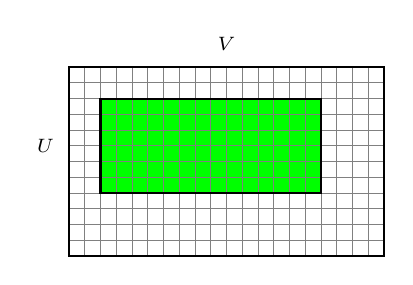
\begin{tikzpicture}
    \draw[fill = green] (0.4, -0.4) rectangle (3.2, -1.6);
    \draw[step = 0.2, gray, thin] (0, 0) grid (4, -2.4);
    \draw[black, thick] (0, 0) rectangle (4, -2.4);
    \draw[black, thick] (0.4, -0.4) rectangle (3.2, -1.6);
    \node at (-0.3, -1.) {\scriptsize $U$};
    \node at (2, 0.3) {\scriptsize $V$};
\end{tikzpicture}

    \end{center}

    We need \alert{triangles} instead of rectangles.

\end{frame}

\begin{frame}{Proof Idea}

    \begin{itemize}
        \item $\mu\colon X \cup Y \to H$ (partial mapping);
        \item $|\Dom(\mu)| = \Omega(\min(|X|, |Y|)) = 2^{n - \bigO{1}}$;
        \item $\forall h \in H, |\mu^{-1}(h)| \le 2^{n - f(n)}$.
    \end{itemize}

    \pause
    Idea: $\mu(x) = h \Leftrightarrow h$ is the bottommost node where $R_h$ contains ``useful
    information'' about $x$.

    \pause

    \begin{minipage}{0.38\linewidth}
        \centering
        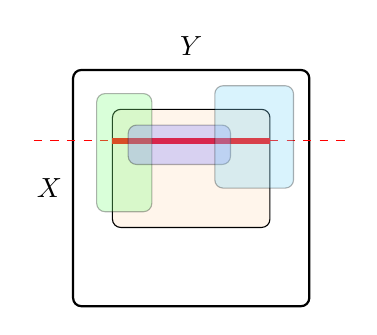
\begin{tikzpicture}
    \draw[thick, rounded corners = 3pt] (0, 0) rectangle (3, -3);
    \draw[fill = orange!8, rounded corners = 3pt] (0.5, -0.5) rectangle (2.5, -2);
    \node at (-0.3, -1.5) {$X$};
    \node at (1.5, 0.3) {$Y$};

    \draw[red, dashed] (-0.5, -0.9) -- (0.5, -0.9);
    \draw[line width = 2pt, red] (0.5, -0.9) -- (2.5, -0.9);
    \draw[red, dashed] (2.5, -0.9) -- (3.5, -0.9);

    \pause
    \only<2->{
        \draw[fill = green!50, rounded corners = 3pt, opacity = 0.3] (0.3, -0.3) rectangle (1, -1.8);
        \draw[fill = blue!50, rounded corners = 3pt, opacity = 0.3] (0.7, -0.7) rectangle (2, -1.2);
        \draw[fill = cyan!50, rounded corners = 3pt, opacity = 0.3] (1.8, -1.5) rectangle (2.8, -0.2);
    }

    \onslide<1->
\end{tikzpicture}

    \end{minipage}
    \begin{minipage}{0.58\linewidth}
        \pause
        \begin{itemize}
            \item $w(h, x_0) \coloneqq$ size of minimal monochr. covering
            \item $k \coloneqq n / \log(n)$
            \item $\mu(x_0) =$ the bottommost $h$ such that $w(h, x_0) \ge k$.
        \end{itemize}
    \end{minipage}

\end{frame}

\begin{frame}{Definition of $\mu$}

    \begin{minipage}{0.6\linewidth}
        \begin{enumerate}
            \item For all $h \in H$ from leafs to root.
                \pause
            \item $\forall x \in X, w(h, x) > k \Rightarrow$
                \begin{itemize}
                    \item $\mu(x) \coloneqq h$;
                    \item erase $\{x\} \times Y$ from \alert{all} rectangles in $H$.
                \end{itemize}
            \item $\forall y \in X, w(h, y) > k \Rightarrow$
                \begin{itemize}
                    \item $\mu(y) \coloneqq h$;
                    \item erase $X \times \{y\}$ from \alert{all} rectangles in $H$.
                \end{itemize}
                \pause
            \item Goto next $h$.
        \end{enumerate}
    \end{minipage}    
    \begin{minipage}{0.36\linewidth}
        \centering
        
\includegraphics[scale = 0.1]{pics/utia-fly.png}
    \end{minipage}

    \begin{lemma}
        At current node $h$
        \begin{itemize}
            \item before: $\forall z \in X \cup Y, w(h, z) \le 2k$;
            \item after: $\forall z \in X \cup Y, w(h, z) \le k$.
        \end{itemize}
    \end{lemma}
\end{frame}

\begin{frame}{First property}
    \begin{lemma}
        $|\Dom(\mu)| \ge \min(|X|, |Y|) / 2$.
    \end{lemma}
    \begin{proof}

        \pause
        \begin{center}
            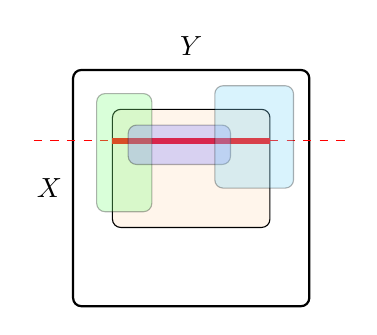
\begin{tikzpicture}
    \draw[thick, rounded corners = 3pt] (0, 0) rectangle (3, -3);
    \draw[fill = orange!8, rounded corners = 3pt] (0.5, -0.5) rectangle (2.5, -2);
    \node at (-0.3, -1.5) {$X$};
    \node at (1.5, 0.3) {$Y$};

    \draw[red, dashed] (-0.5, -0.9) -- (0.5, -0.9);
    \draw[line width = 2pt, red] (0.5, -0.9) -- (2.5, -0.9);
    \draw[red, dashed] (2.5, -0.9) -- (3.5, -0.9);

    \pause
    \only<2->{
        \draw[fill = green!50, rounded corners = 3pt, opacity = 0.3] (0.3, -0.3) rectangle (1, -1.8);
        \draw[fill = blue!50, rounded corners = 3pt, opacity = 0.3] (0.7, -0.7) rectangle (2, -1.2);
        \draw[fill = cyan!50, rounded corners = 3pt, opacity = 0.3] (1.8, -1.5) rectangle (2.8, -0.2);
    }

    \onslide<1->
\end{tikzpicture}

        \end{center}

        \pause
        \begin{align*}
          w(\mathrm{root}, x_0) \le k & \Rightarrow
                                        \exists S \subseteq \varphi, |S| \le k: \forall y
                                        \in Y_{\mathrm{root}}, S(x_0, y) = 0 \\
                                      & \Rightarrow |Y_{\mathrm{root}}| \le k / 2^{\Delta} \cdot |Y|.
        \end{align*}
    \end{proof}    
\end{frame}


\begin{frame}{Expansion}

    \begin{minipage}{0.38\linewidth}
        \centering
        \begin{tikzpicture}

    \pgfmathsetseed{1000007}
    \foreach \i in {0, 1, ..., 4}{
        \node[graph-vert] (b\i) at (1.5, 0.4 * \i - 2.5 * 0.4) {};
    }


    \foreach \i in {0, 1, ..., 8}{
        \node[graph-vert = {LEIorange!80!black}{0.15cm}] (a\i) at (0,
        0.4 * \i - 4.5 * 0.4) {};
    }

    \uncover<1-3>{
        \draw (a3) -- (b1);
        \draw (a3) -- (b2);
        \draw (a3) -- (b3);
        \draw (a4) -- (b3);
        \draw (a4) -- (b4);

        \fill[rounded corners = 3pt, orange, opacity = 0.2]
            (-0.2, -0.8) rectangle (0.2, 0);
        \draw[rounded corners = 3pt, orange, thick] (-0.2, -0.8)
            rectangle (0.2, -0);

        \fill[rounded corners = 3pt, blue!80!black, opacity = 0.2]
            (1.3, -0.8) rectangle (1.7, 0.8);
        \draw[rounded corners = 3pt, blue!80!black, thick] (1.3, -0.8)
            rectangle (1.7, 0.8);

        \node at (-0.4, -0.4) {$S$};
        \node at (2.25, 0) {$\mathrm{N}(S)$};
    }

    \uncover<5->{
        \fill[rounded corners = 3pt, blue!80!black, opacity = 0.2]
            (1.33, 0) rectangle (1.67, 0.8);
        \draw[rounded corners = 3pt, blue!80!black, thick] (1.33, 0)
            rectangle (1.67, 0.8);
        \node at (2.27, 0.4) {$J$};        
    }

    \uncover<6->{
        \draw (a3) -- (b2);
        \draw (a3) -- (b3);
        \draw (a4) -- (b3);

        \fill[rounded corners = 3pt, orange, opacity = 0.2]
            (-0.2, -0.8) rectangle (0.2, 0);
        \draw[rounded corners = 3pt, orange, thick] (-0.2, -0.8)
            rectangle (0.2, -0);
        \node at (-0.4, -0.4) {$I_J$};
    }
    \uncover<7->{
        \fill[rounded corners = 3pt, orange, opacity = 0.2]
            (1.28, -0.4) rectangle (1.72, 0.4);
        \draw[rounded corners = 3pt, orange, thick] (1.281, -0.4)
            rectangle (1.72, 0.4);
        \node at (2.27, 0) {$\mathrm{N}(I)$};
    }
        
\end{tikzpicture}
    \end{minipage}
    \begin{minipage}{0.58\linewidth}
        \begin{itemize}
            \item $(r, \Delta, c)$-expander;
            \item $\forall S \subseteq L, |S| \le r \Rightarrow$
                \begin{itemize}
                    \item $\mathrm{N}_{X}(S) \ge c |S|$;
                    \item $\mathrm{N}_{y}(S) \ge c |S|$.
                \end{itemize}
        \end{itemize}
    \end{minipage}
\end{frame}

\begin{frame}
    \begin{lemma}
        $\forall h \in H, |\mu^{-1}(h)| \le 2^{n - \Omega(k \log k)}$.
    \end{lemma}

    \pause

    \begin{proof}
        
        \begin{minipage}{0.38\linewidth}
            \centering
            \begin{tikzpicture}
    \draw[thick, rounded corners = 3pt] (0, 0) rectangle (3, -3);
    \draw[fill = orange!8, rounded corners = 3pt] (0.5, -0.5) rectangle (2.5, -2.5);
    \node at (-0.3, -1.5) {$X$};
    \node at (1.5, 0.3) {$Y$};

    \draw[red, dashed] (0.6, 0.3) -- (0.6, -0.5);
    \draw[red, line width = 2pt] (0.6, -0.5) -- (0.6, -2.5);
    \draw[red, dashed] (0.6, -2.5) -- (0.6, -3.3);

    \pause
    \only<3->{
        \draw[fill = green!50, rounded corners = 3pt, opacity = 0.3] (0.3, -0.3) rectangle (1.4, -1.8);
        \draw[fill = blue!50, rounded corners = 3pt, opacity = 0.3] (0.4, -1.5) rectangle (1, -2.2);
        \draw[fill = cyan!50, rounded corners = 3pt, opacity = 0.3] (0.2, -2.1) rectangle (0.8, -2.6);
    }

    \pause
    \only<4->{
        \draw[fill = black!80] (1.4, -0.5) {[rounded corners = 3pt] -- (2.5, -0.5)} -- (2.5, -1.8) -- (1.4, -1.8) -- cycle;
    }

    \pause
    \only<5->{
        \draw[red, dashed] (1.5, 0.3) -- (1.5, -0.5);
        \draw[red, line width = 2pt] (1.5, -0.5) -- (1.5, -1.8);
        \draw[red, dashed] (1.5, -1.8) -- (1.5, -3.3);
    }

    \pause
    \only<6->{
        \draw[fill = white!50, rounded corners = 3pt, opacity = 0.3] (1.4, -0.4) rectangle (1.8, -0.6);
        \draw[fill = white!50, rounded corners = 3pt, opacity = 0.3] (1.4, -0.6) rectangle (1.8, -1);
        \draw[fill = white!50, rounded corners = 3pt, opacity = 0.3] (1.4, -0.9) rectangle (1.7, -2);
        
    }
        

    \onslide<1->
\end{tikzpicture}

        \end{minipage}
        \begin{minipage}{0.58\linewidth}
            \centering
            \begin{tikzpicture}

    \node[graph-vert] (t0) at (0, 0) {};
    \node at (-3, 0) {};
    \node at (1.8, -2.9) {};

    %\pause
    \only<3->{
        \foreach \i in {1, 2, 3}{
            \node[graph-vert] (t1\i) at (1.2 * \i - 2.4, -1) {};
            \draw (t0) -- (t1\i);
        }
        \draw[blue, <->] (-10:0.5) arc (-10:-170:0.5) node[below left] {$\le 2k$};
    }

    \only<6->{
        \foreach \i in {1, 2, 3}{
            \node[graph-vert] (t2\i) at (\i - 3.4, -2) {};
            \draw (t11) -- (t2\i);
        }

        \draw[blue, <->] (t11) ++(-10:0.5) arc (-10:-170:0.5) node[below left] {$\le 2k$};
    }
    
    \pause
    \only<7->{
        \node (t) at (-2.9, -2.7){$\vdots$};
        \draw (t21) -- (t);

        \draw[<->] (1.5, 0) -- (1.5, -3) node[midway, right] {$k$};
    }   
        
    \onslide<1->
\end{tikzpicture}

        \end{minipage}

        \pause
        \begin{itemize}
            \item $x_0 \in $ leaf $\Rightarrow \exists S \subseteq \varphi, |S| \le k, x_0$ do not
                satisfy \alert{any} clause in $S$.
            \item Expansion in $X$ $\Rightarrow$ at most $2^{n - ck}$ such $x$.
            \item There are at most $(2k)^k$ leaves.
            \item Altogether: $|\mu^{-1}(h)| \le 2^{n - ck + k \log 2k}$ 
        \end{itemize}
    \end{proof}
\end{frame}

\begin{frame}{Open Problems: Nisan--Wigderson Generators (naive encoding)}

    \begin{minipage}{0.48\linewidth}
        \centering
        \begin{tikzpicture}

    \pgfmathsetseed{1000007}
    \foreach \i in {0, 1, ..., 5}{
        \node[graph-vert] (b\i) at
            (1.5, 0.4 * \i + 0.4) {};
    }

    \foreach \i in {0, 1, ..., 7}{
        \node[graph-vert = {LEIorange!80!black}{0.15cm}] (a\i) at
            (0, 0.4 * \i) {};

        \draw[->] (a\i) -- ++(-0.3, 0);

        \foreach \j in {0, 1, 2}{
            \pgfmathsetmacro{\temp}{random(0, 5)}
            \draw (a\i) -- (b\temp);
        }
    }

    \node[below = 0.2cm] at (a0) {$m$};
    \node[below = 0.2cm] at (b0) {$n$};
\end{tikzpicture}
    \end{minipage}
    \putpos{-40}{50}{
\includegraphics[scale = 0.1]{pics/utia-rest.png}}
    \begin{minipage}{0.48\linewidth}
        \begin{itemize}
            \item $\Delta$ is the left degree;
            \item $P(x_1, \dots, x_{\Delta})$ is a predicate.
        \end{itemize}
        
        \vspace{0.2cm}
        \pause
        \begin{itemize}
            \item Strategy do not work for balanced predicates;
            \item Upper bound if $P$ is $\Parity$;
            \item $\Ppoly$ vs $\NP$;
        \end{itemize}
    \end{minipage}
\end{frame}

\begin{frame}{Open problems}

    \begin{itemize}
        \item PRG. Other encodings.
        \item $\bigO{1}$-random CNF.
        \item ``Sepataion'' betweem CP and monotone circuits.
    \end{itemize}

    \vspace{1cm}
    \centering
    
\includegraphics[scale = 0.1]{pics/utia-think.png}
\end{frame}